% !TEX root = ../0_tcc.tex

\begin{figure}[H]
	\centering
	\begin{subfigure}{\textwidth}
		\centering
		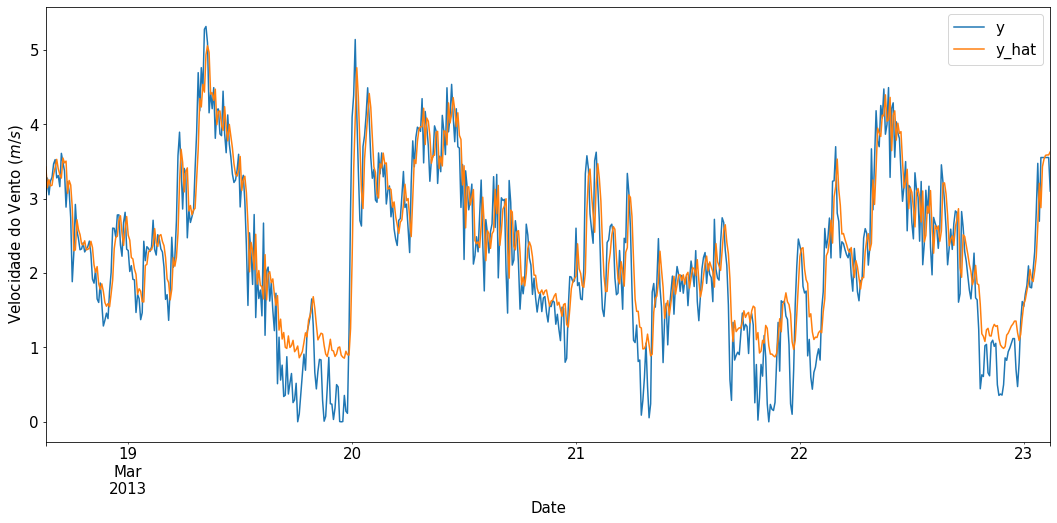
\includegraphics[width=0.7\textwidth]{../img/wind_pred_3m_0.png}
		\caption{Previsão realizada pela primeira rede}\label{fig:wind:pred1}
	\end{subfigure}
	\\ \vspace{1cm}
	\begin{subfigure}{\textwidth}
		\centering
		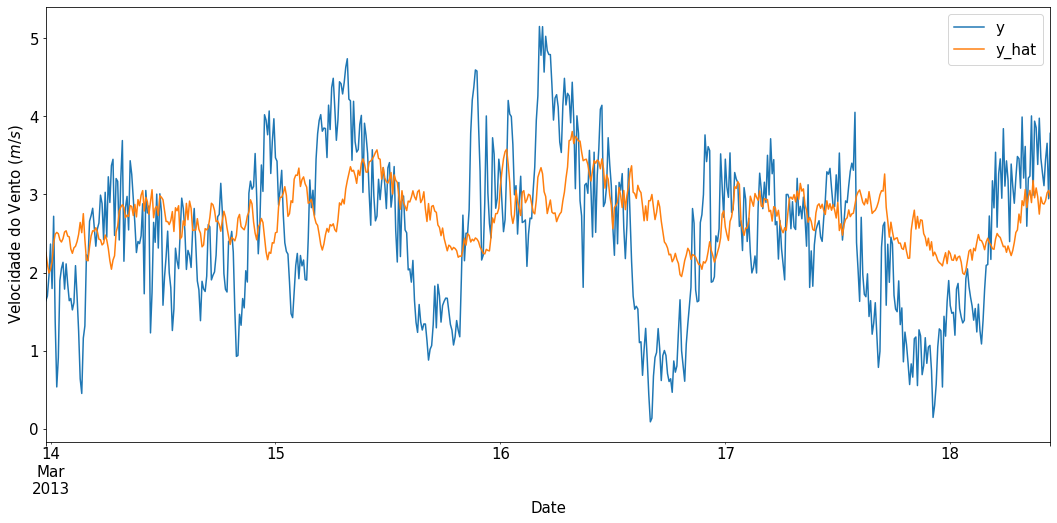
\includegraphics[width=0.7\textwidth]{../img/wind_pred_3m_18.png}
		\caption{Previsão realizada pela décima oitava rede}\label{fig:wind:pred18}
	\end{subfigure}
	\\ \vspace{1cm}
	\begin{subfigure}{\textwidth}
		\centering
		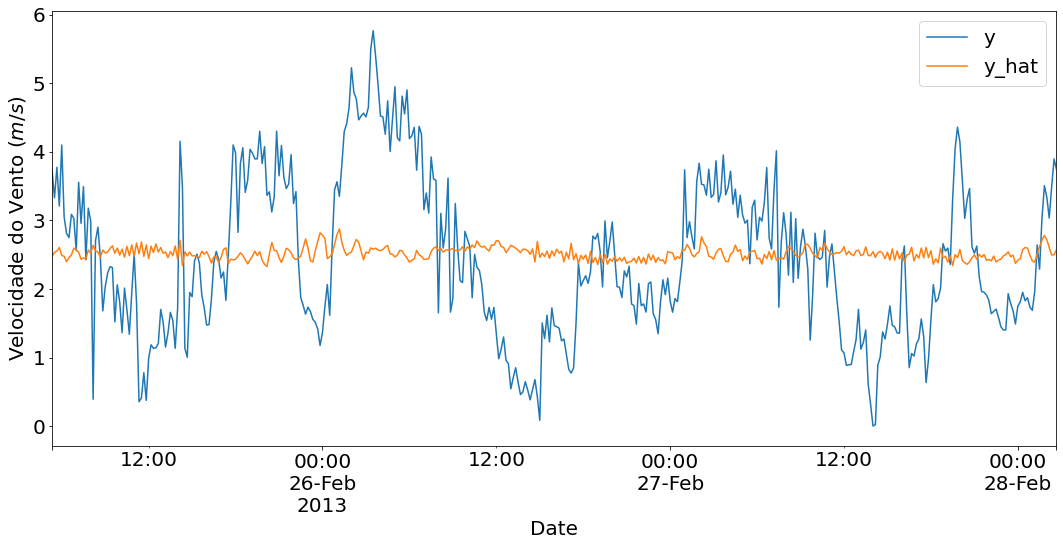
\includegraphics[width=0.7\textwidth]{../img/wind_pred_3m_-1.png}
		\caption{Previsão realizada pela última rede}\label{fig:wind:pred-1}
	\end{subfigure}
	\caption{Previsão de velocidade do vento nos dados de teste}\label{fig:wind:pred}
\end{figure}
